% !TEX root = ../main.tex

Inicialmente, foi necessário entender o problema do qual seria tratado, traçar características e definir uma visão com o cliente para impedir problemas futuros, como, por exemplo, problemas de comunicação causados por ambiguidade, estas informações estão esclarecidas no Documento de Visão, presente na Sessão \ref{sec:document_de_visao} deste documento.

Após a definição do Problema iniciou-se a parte de elicitação de requisitos, tanto funcionais como não funcionais, a modelagem desta está representada na Figura \ref{img:modelagem1}.

\begin{figure}[H]
	\centering
	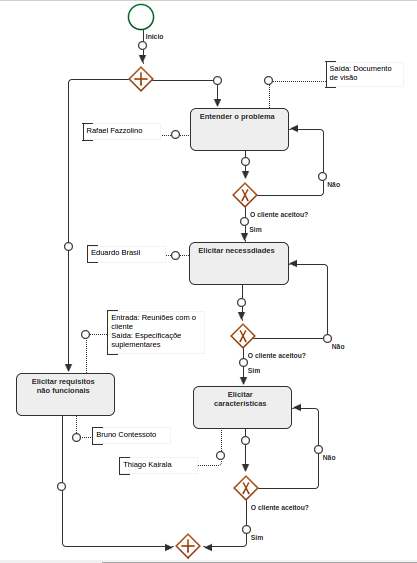
\includegraphics[width=0.8\textwidth]{imgModelagem/modelagem1}
	\caption{Modelagem de processo parte 1}
	\label{img:modelagem1}
\end{figure}


Após a definição dos casos de uso do projeto, deve-se definir as prioridades, criação dos \textit{roadmaps}, assim como detalhamento dos casos de uso e implementação das funcionalidades com maior prioridade do projeto, porém, durante o andamento, já estavam definidos os casos de uso que seriam implementados na primeira entrega, então foi feito em paralelo o plano de iteração e o primeiro \textit{roadmap}. A modelagem do mesmo esta presente na Figura \ref{img:modelagem2}.

O detalhamento dos casos de uso está presente na Sessão \ref{sec:documento_de_caso_de_uso} deste documento, assim como os \textit{roadmaps} se encontram na Sessão \ref{sec:road_map}.

\begin{figure}[H]
	\centering
	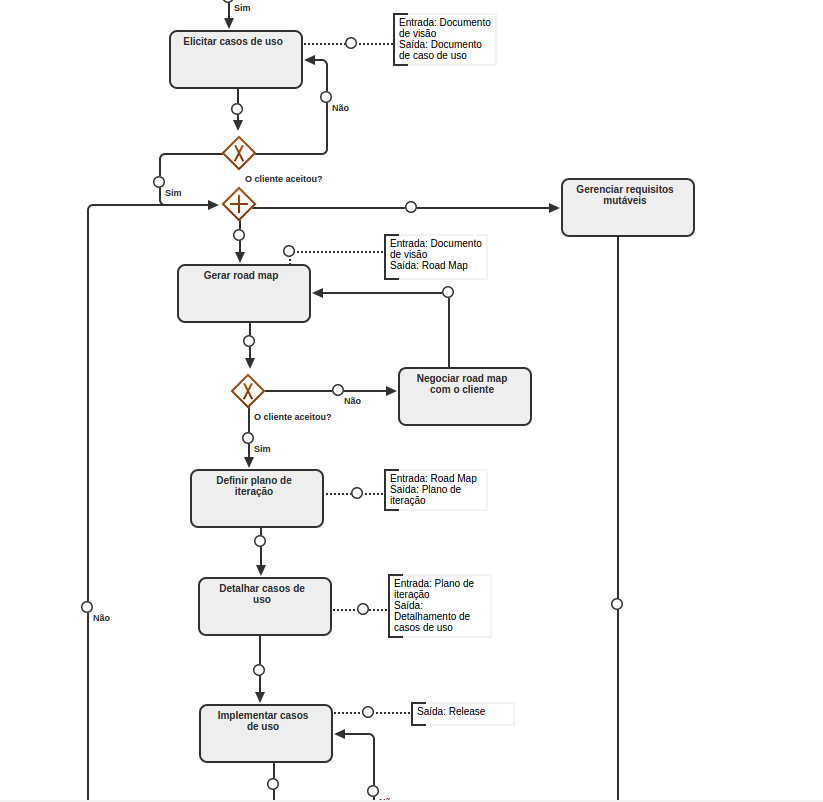
\includegraphics[width=1\textwidth]{imgModelagem/modelagem2}
	\caption{Modelagem de processo parte 2}
	\label{img:modelagem2}
\end{figure}

Após a implementação dos casos de uso da iteração, caso o cliente aceite, segue-se para a próxima iteração ou final do projeto, dependendo se existe ou não outros casos de uso a serem implementados, caso haja, o processo volta para as atividades de gerar o \textit{road map}  e gerenciar requisitos mutáveis presentes na Figura \ref{img:modelagem2}, assim como mostra a Figura \ref{img:modelagem3}.

\begin{figure}[H]
	\centering
	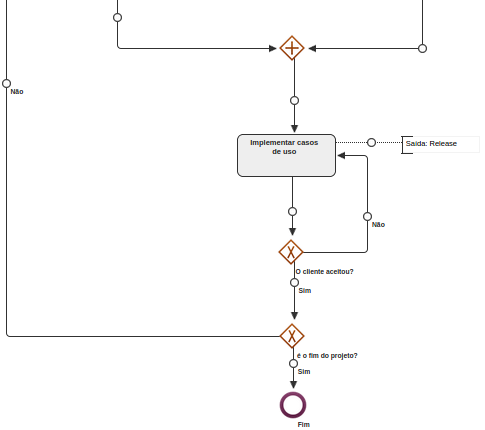
\includegraphics[width=1\textwidth]{imgModelagem/modelagem3}
	\caption{Modelagem de processo parte 3}
	\label{img:modelagem3}
\end{figure}
